\documentclass[12pt]{beamer}
\usetheme{metropolis}           % Use metropolis theme
\metroset{titleformat=smallcaps}

\usepackage[utf8]{inputenc}
\usepackage[T1]{fontenc}
\usepackage{textcomp}
% \usepackage{amsmath,amsfonts,amssymb}
\usepackage{url}

% disable Navigation at the bottom
\beamertemplatenavigationsymbolsempty

% Cool font
\usepackage{FiraSans}
% \usepackage[sfdefault,light]{FiraSans}
% \usepackage{newtxsf}

% page numbers
% \setbeamertemplate{footline}[frame number]
% \setbeamertemplate{footline}
% \setbeamertemplate{headline}

% style for source code
\usepackage{listings}
\newcommand{\Hilight}{\makebox[0pt][l]{\color{light-gray}\rule[-4pt]{1.0\linewidth}{12pt}}}
\usepackage{color}
\definecolor{light-gray}{gray}{0.80}
  
% use {\mono lorem} to set something in monospace
\newcommand{\mono}[1]{\ttfamily\fontsize{14}{14}\selectfont #1}

% wanna use Metapost?
\makeatletter
\newcommand\@ptsize{12}
\makeatother

\usepackage{mflogo}
\usepackage{emp}
\DeclareGraphicsRule{*}{mps}{*}{}


\title{Disposition 4: Network Security Mechanisms}   
\author{Mathias Ravn Tversted} 
\date{\today} 

% Definition of AKE

% Needham/Schroeder and the attack

% SSL/TLS and the SSL handshake
    % Why is it secure
    % One-way SSL

% Diffie-Hellman key exchange and IPSec

% Difference between SSL and IPSec

% Password authenticated key exchange

% Applications, document based secure formats versus secure tunnels

%===================================
\begin{document}

\frame{\titlepage} 

\frame{\frametitle{Table of contents}\tableofcontents} 
%===================================
    \section{Authenticated Key Exchange}
        \frame{\frametitle{Definition of AKE}
            An \textit{authenticated key exchange protocol} is a protocol for two parties $A, B$. Each party starts the protocol with the intention of establishing a key with some other party. At the end, each party outputs either "accept" or "reject" as well as a key. The protocol is said to be secure if the three conditions hold.
        }

        \frame{\frametitle{Agreement}
            \textbf{Agreement}: Assume that $A$ intends to talk to $B$ and vice versa. Assume also that both parties accept $A$ and outputs key $K_A$ while $B$ outputs key $K_B$, then $K_A = K_B$. 
        }
        \frame{\frametitle{Secrecy and Authentication}
            \textbf{Secrecy and Authentication}: Assume $A$ intends to talk to $B$, and accepts. Then it must be the case that $B$ participated in the protocol and if $B$ also accepts, he did indeed intend to talk to $A$. Furthermore, the adversary does not know the key $K$ that $A$ outputs. A symmetric condition holds for $B$.
        }
        \frame{\frametitle{Freshness}
            \textbf{Freshness}: if $A(B)$ follows the protocol and accepts, it is guaranteed that the key $K$ that is output is a fresh key, i.e., it has been randomly chosen for this instance of the protocol, independently of anything else.
        }
        \frame{\frametitle{About AKE}
                These properties give us some desirable properties, such as the preventing the following attacks: 
                \begin{itemize}
                    \item Adversary cannot stop last message in the protocol for party $A$ but not party $B$
                    \item Freshness means adversary cannot trick you into using old key
                    \item Worst thing adversary can do is attempt to block communication
                \end{itemize}
        }
%===================================

    \section{Needham-Schröder Attack}
                \frame{\frametitle{The N-S protocol}
                    \begin{enumerate}
                        \item A chooses nonce $n_A$ and sends $E_{pk_B}(ID_A, n_A)$ to $B$.
                        \item B decrypts, checks $ID_A$, chooses nonce $n_B$ and sends $E_{pk_A}(n_A, n_B)$ to $A$. 
                        \item $A$ decrypts and checks that the correct value of $n_A$ appears in the result, and sends $E_{pk_B}(n_B)$ to $B$. 
                        \item B decrypts and checks that the correct value of $n_B$ appears in the result.
                        \item If the checks are executed are OK, each party computes the session key as some fixed function of $n_A, n_B$. 
                    \end{enumerate}
                }
                \begin{frame}
                    If some third-party $E$ has a certified public key, they can mix two instances of the protocol and fool $B$.  

                    \begin{enumerate}
                        \item A starts a session with $E$. $A$ sends $E_{pk_E}(ID_A, n_A)$ to $E$
                        \item $E$ decrypts this and starts session with $B$, pretending to be $A$. $E$ sends $E_{pk_B}(ID_A, n_A) to B$
                        \item $B$ decrypts and finds the right ID and sends $E_{pk_A}(n_A, n_B)$ to $E$
                        \item E is not able to decrypt, but forwards message $E_{pk_A}(n_A, n_B)$ to $A$
                        \item $A$ will decrypt, and find an expected result, and will return $E_{pk_E}(n_B)$ to $E$
                        \item $E$ can decrypt it, find $n_B$ and can send $E_{pk_B}(n_B)$ to $B$
                        \item When $B$ decrypts it, he can will accept because it's  the right value of $n_B$. 
                    \end{enumerate}
                \end{frame}

%===================================

    \section{SSL/TLS}
                \begin{frame}
                    \frametitle{SSL and TLS}
                    SSL protocol for authenticated key exchange
                    \begin{itemize}
                        \item Uses digital signatures in addition to encryption, as opposed to Needham-Schroeder
                        \item Basic idea: Party must sign a nonce chosen by the other
                        \item Replaced by Transaction Layer Security (TLS), but still refered to as SSL 
                        due to minor differences
                        \item SSL is secure against the Needham-Schroeder attack
                        \item SSL sits between application and TCP/IP Transport Layers
                    \end{itemize}
                \end{frame}

                \begin{frame}
                    \frametitle{SSL protocols}
                    SSL is compromised of the followng protocols
                    \begin{itemize}
                        \item \textbf{Record Protocol}: Responsible for "raw" transmission of data. \textit{cipher spec} determines what kinds of encryption algorithms to use
                        \item \textbf{Handshake protocol}: The part of SSL that does the authenticated key exchange
                        \item \textbf{Change cipher spec protocol}: Changes the cipher spec
                        \item \textbf{Alert protocol}: Error messages
                    \end{itemize}
                \end{frame}

                \begin{frame} 
                    \frametitle{One-sided SSL Handshake}
                        \begin{itemize}
                            \item Client picks random $n_C$
                            \item Server picks random $n_S$
                            \item Server sends $n_S, Cert_S$
                            \item Client picks random $pms$, sends $E_{pk_S}(pms)$
                            \item Server computes $K = f(pms, n_C, n_S)$ and sends $MAC_K(view_S)$
                            \item Client sends $MAC_K(view_C)$
                        \end{itemize}
                \end{frame}

                \begin{frame}
                    \frametitle{Handshake Protocol}
                        The actual key-exchange protocol worksas follows. This is but one of the variations of the handshake protocol
                        \begin{itemize}
                            \item $C$ sends a hello message containing nonce $n_C$
                            \item $S$ sends a nonce $n_S$ and its certificate $Cert_S$ (containing public key $pk_S$ of $S$)
                            \item $C$ verifies $Cert_S$ and chooses a so called pre master secret \textit{pms} at random. $C$ sends $E_{pk_S}(pms)$ to $S$, also $C$ sends its certificate $Cert_C$ to $S$, plus its signature $sig_C$ on the concat of $n_C, n_S$ and $E_{pk_S}(pms)$
                            \item $S$ verifies $Cert_C$ and $sig_C$. If OK; it decrypts \textit{pms}. 
                            \item $S$ sends to $C$ a "finished" message containing essentially a MAC all messages he has sent and received sent in this instance of the protocol, with \textit{pms} the secret key.
                            \item $C$ verifies the MAC, and if OK returns its own finished message to $S$, also with a MAC on all messages sent and received up to this step (note that this now includes the finished message from $S$, so one cannot just repeat the previous message). $S$ verifies the MAC when it is received.
                            \item At this point both parties derive from $n_S,n_C$ and \textit{pms} a set of keys for secret-key authentication and encryption of the following data exchange. Typically this is done using a hash function.
                        \end{itemize}
                \end{frame}
            \begin{frame}
                \frametitle{Handshake Protocol}
                    \begin{itemize}
                        \item $S$ sends to $C$ a "finished" message containing essentially a MAC all messages he has sent and received sent in this instance of the protocol, with \textit{pms} the secret key.
                        \item $C$ verifies the MAC, and if OK returns its own finished message to $S$, also with a MAC on all messages sent and received up to this step (note that this now includes the finished message from $S$, so one cannot just repeat the previous message). $S$ verifies the MAC when it is received.
                        \item At this point both parties derive from $n_S,n_C$ and \textit{pms} a set of keys for secret-key authentication and encryption of the following data exchange. Typically this is done using a hash function.
                    \end{itemize}
            \end{frame}
            \begin{frame}
                It is important to point out that there are MAC's on all messages sent. This means that the attacker cannot modify messages sent. This doesn't prove that the interleaving attack doesn't work. 
            \end{frame}
            \begin{frame}
                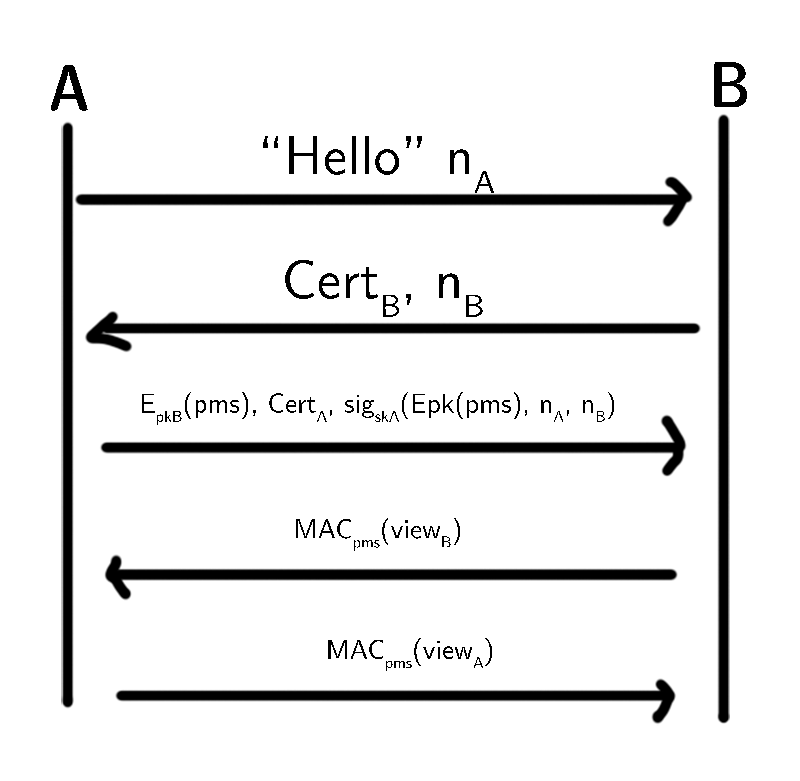
\includegraphics[width=0.8\textwidth]{content/ssl.pdf}
            \end{frame}

            \begin{frame}
                \frametitle{Why is it correct}
                    Consider honest client $C$ who wants to talk to $S$. $C$ sends \textit{pms} encrypted under $pk_S$.
                    Only $S$ will be able to decrypt this. 
                    Protocol never asks $S$ for \textit{pms} 
                    When $C$ receives a message with a MAC that verifies using pms, he knows this MAC comes from $S$. 
                    The MAC can be verified w.r.t. all messages $C$ has sent and received it must be the case that $S$ has seen this same of messages on his side. 
                    An adversary that sits between $C$ and $S$ can have done nothing except forward all messages unchanged. 
                    Conversely, let us see things from the point of view of an honest $S$ who wants to talk to $C$. He sees a signature from $C$ on a ciphertext $c$ and the nonces, and since he chose one of the nonces himself, he knows the signature and hence c was indeed produced now by $C$, i.e., it is not a replay. Furthermore, an honest $C$ will send a \textit{pms} to only one server, and $S$ will not himself send pms to anyone. Therefore, when $S$ receives a message with a MAC that verifies using pms, he knows this MAC comes from $C$. If furthermore the MAC can be verified w.r.t. all messages $S$ has sent and received it must be the case that $C$ has seen this same of messages on his side. Therefore, as above, any adversary that sits between $C$ and $S$ can have done nothing except forward all messages unchanged.
            \end{frame}

%===================================
\section{Diffie Hellman and IPSEC}
% Diffie-Hellmann and IPSEC
    \begin{frame}
        \frametitle{IPSEC}
            \begin{itemize}
                \item Sits on Transport Layer
                \item Sets up secure connection, known as \textit{Security Association}
                \item \textit{Internet Key Exchange} (IKE)
                \item IKE is independent of IPSEC
                \item Mostly uses the \textit{Diffie-Hellman Key Exchange}
            \end{itemize}
    \end{frame}

    \begin{frame}
           \frametitle{(Authenticated) Diffie-Hellmann Key Exchane}
            Choose $g \in [0, p-1]$. Then execute the following protocol
            \begin{itemize}
                \item $C$ chooses a random number $a$ and sends $g^a \mod p$ and certificate to $S$. 
                \item $S$ chooses $b$ and sends $g^b \mod p$ and certificate to $C$
                \item $C$ computes $(g^b \mod p)^a \mod p$ based on what he got from $S$ and sends own random choice
                \item $S$ computes $(g^a \mod p)^b \mod p$ These values are equal to $g^{ab} \mod p$. This is now the common key
                \item $C, S$ sign all messages they have seen so far and send them to each other
                \item If both verify, then everything is OK
            \end{itemize}
            Vulnerable to preprocessing attack \textit{Index Calculus} algorithm. So choose fresh primes.
    \end{frame}

    \begin{frame}
        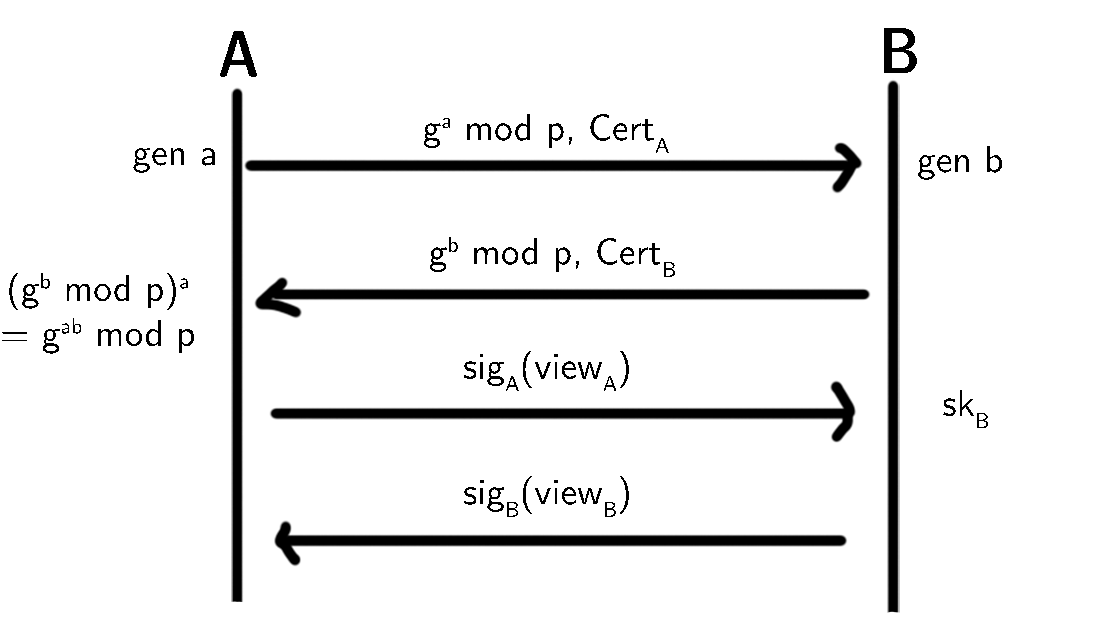
\includegraphics[width=0.8\textwidth]{content/diffie-helmann.pdf}
    \end{frame}

%===================================
\section{Difference between SSL and IPSEC}
% Difference between SSL and IPSEC

    \begin{frame}
        \frametitle{Difference between SSL and IPSEC}
        % PUT DETTE HER LÆNGERE OP ET STED HVOR DET ER RELEVANT OG TAL OM HVAD DER ER OG HVAD DER IKKE ER FORWARD SECURE
        \textbf{Forward Security definition}: "Forward security means that the security of the session you do now cannot be compromised even if the adversary steals a long-term secret key some time in the future"
        \begin{itemize}
            \item SSL protects applications, even from other applications or users on the machine
            \item Applications must know how to use SSL
            \item IPSEC protects \textit{all} applications, even if they are not aware of it. 
            \item Data is always never secure once it leaves the encrypted tunnels
            \item SSL allows one-way authentication, so that the client doesn't need a certificate
            \item But client can use a password
        \end{itemize}
    \end{frame}

    \begin{frame}
        \frametitle{Password authenticated key exchange}
            Password authenticated key exchange can be used to authenticate a user, so it's not just secure, but also the client is authenticated. The following is based on Diffie-Hellmann and is a simplified version of Bellare et al.
            \begin{itemize}
                \item $C$ chooses random number $a$ and sends $A = E_{pw}(g^a \mod p)$
                \item $S$ chooses $b$ at random and sends $B = E_{pw}(g^b \mod p)$
                \item $C$ decrypts $B$ with password $pw$ and computes $(g^b \mod p)^a \mod p$ based on result of decryption and his own random choice
                \item $S$ computes $(g^a \mod p)^b \mod p$. These are equal and can be used as common key
                \item The parties then continue verifying and confirming like in Diffie Hellmann
            \end{itemize}
            Since adversary cannot easily verify guess. This is protected against dictionary attacks. 

    \end{frame}


%===================================
% Applications, document based secure formats versus secure tunnels
    \begin{frame}
        \frametitle{Applications, document based secure formats versus secure tunnels}
            Indsæt stuff her. Sikkert ikke tid til det
    \end{frame}


\end{document}

